\documentclass{article}

\usepackage[margin=1in]{geometry}
\usepackage[utf8]{inputenc}
\usepackage[parfill]{parskip}
\usepackage{amsmath}
\usepackage{amsfonts}
\usepackage{caption}
\usepackage{graphicx}
\usepackage{subcaption}
\usepackage{algorithm2e}
\usepackage{epsfig}
%\usepackage{subfigure}

\title{Learning from (multiple) demonstrations through robust trajectory transfer}
\author{Alex Lee, Dylan Hadfield-Menell, Eric Tzeng, Sandy Huang}
\date{}

\renewcommand{\thesection}{\Roman{section}}
\renewcommand\thesubsection{\Alph{subsection}}
%\renewcommand{\thesubsection}{\thesection.\Roman{subsection}}

% variables used across report
\newcommand*{\xs}[1]{\ensuremath{\mathbf{x}_s^{(#1)}}}
\newcommand*{\xt}[1]{\ensuremath{\mathbf{x}_t^{(#1)}}}
\newcommand*{\xes}[1]{\ensuremath{\mathbf{x}_{e,s}^{(#1)}}}
\newcommand*{\ns}[1]{\ensuremath{\mathbf{n}_s^{(#1)}}}
\newcommand*{\nt}[1]{\ensuremath{\mathbf{n}_t^{(#1)}}}

\DeclareMathOperator{\Tr}{Tr}

\begin{document}

\maketitle

\begin{abstract}
We investigate extensions to a previously presented method of learning from demonstrations via trajectory transfer. We present a detailed overview of the current state-of-the-art and propose a reformulation of the underlying optimization problem to jointly optimize for non-rigid registration and trajectory feasibility. We also discuss an extension which incorporates first-order constraints into the optimization to further preserve important aspects of the scene geometry. Finally, we explore methods in which we use our reformulated optimization problem to enable autonomous robots to complete various manipulation tasks. We demonstrate that our version of this optimization problem improves the quality and success rate of robots in completing these tasks.
\end{abstract}

\section{Introduction}

Robots often have to perform a given task in a variety of scenarios, making it impractical or even impossible to individually specify trajectories for all possible scenarios. \emph{Learning from demonstrations} is an approach that enables robots to generalize from demonstrations of manipulation tasks in order to perform them in new scenarios. We review this method of generalization via trajectory transfer, which makes heavy use of optimization techniques both to determine a non-rigid registration between the demonstration and the test scene, and to solve for trajectories that avoid obstacles while remaining within the physical constraints of the robot.

Additionally, we identify shortcomings in the current state-of-the-art approach to learning via trajectory transfer. Instead of Schulman et al.'s two-step approach to trajectory transfer~\cite{Schulmanetal_ISRR2013}, which first optimizes for a smooth low-cost registration between the scenes, then separately optimizes for a feasible trajectory, we propose a formulation of the optimization problem that folds these two steps into a single, unified objective. We show this unified approach generalizes demonstrations better by satisfying the ultimate goal -- finding a feasible trajectory in the new scene that has a low-cost registration to the demonstration scene and trajectory.

We also find that the straightforward thin-plate spline approach to non-rigid scene registration often discards information about scene geometry that can be crucial to success in certain manipulation tasks such as autonomous suturing in surgical robots. To address this issue, we investigate a reformulation of the underlying optimization problem that incorporates first-order constraints, thereby enforcing the preservation of surface normals. We believe this extension will improve success rates in tasks such as suturing, where the robot's angle of approach to a surface is crucial to its performance.

Finally, we investigate further applications of this method. We show that the registration error, which appears as a term in our objective function, acts as a strong indicator of state similarity. Thus, we can leverage this similarity to uncover structure in our state space by clustering similar states together. Using these clusters, we can identify state configurations that are poorly understood, since such states will lie outside of our clusters. We can then avoid demonstrations that drive the robot into these unrecoverable configurations, thereby improving our likelihood of success.

% old intro begins here
%Robots often have to perform a given task in a variety of scenarios, making it impractical or even impossible to individually specify trajectories for all possible scenarios. \emph{Learning from demonstrations} is an approach that enables robots to generalize from demonstrations of manipulation tasks in order to perform them in new scenarios. We explore approaches that make this generalization via trajectory transfer more robust and improve its application to multiple demonstrations.

%To improve the robustness of trajectory transfer, we use a unified optimization to determine a feasible trajectory in the new scenario. Instead of Schulman et al.'s state-of-the-art two-step approach~\cite{Schulmanetal_ISRR2013}, which first finds the optimal smooth low-cost registration between the scenes and then a feasible trajectory, we propose optimizing for both at once. We show this unified approach generalizes demonstrations better by satisfying the ultimate goal -- finding a feasible trajectory in the new scene that has a low-cost registration to the demonstration scene and trajectory.

%We also incorporate surface normals into the optimization in order to improve robustness. Without explicitly specifying surface normal correspondences, in order to preserve smoothness the optimal warping function often does not match normals. However, this is undesirable in situations such as suturing, where the robot's angle of approach to the surface is crucial to its performance of the task.

%When there are multiple demonstrations of a task, we improve demonstration selection through simulation and forward search. We simulate potential new trajectories in order to avoid selecting demonstrations that drive us into unrecoverable configurations. We identify unrecoverable states by clustering demonstrations with kernelized $k$-means and using cluster consensus among the $k$-nearest neighbors according to registration cost.
% end old intro

\section{Background}
In this section, we provide an overview of three techniques that our project builds on.
\subsection{Trajectory Optimization through Sequential Convex Programming}
In a trajectory optimization problem, our goal is to find a sequence of controls to move a
robot or dynamic system into a desired state. We would like to minimize some cost on the
trajectory while adhering to the constraints that the path be feasible and collision free.
A trajectory optimization problem can be described by a tuple:$$\langle X, U, O, x_0, G, f, c_T\rangle.$$
Where $X$ is a set of states that our robot can inhabit and $U$ is a set of controls. $O \subset X$ is a set of
states that must be avoided---typically this will be the volume of space occupied 
by obstacles. $x_0 \in X$ is our initial state, and $G\subset X$ is a goal set.
$f: X \times U \rightarrow X$ is a function that describes the dynamics of our problem, so that 
$f(x', u) = x''$ means that applying the control $u$ in state $x'$ will take our robot to state $x''$.
$c_T: (X \times U)^T \rightarrow \mathbb{R} $ is a cost function that measures the cost associated with 
a sequence of controls and states. An example cost function might be deviation from a target trajectory or
the length of the trajectory. With this terminology, we can formalize trajectory optimization
as the following constrained optimization problem:
\begin{align*}
 &\underset{x_1,\ldots, x_T, u_1,\ldots, u_T}{\text{minimize\ \ \ }} & c_T(\{x_i, u_i\}) \\
 &\text{subject to\ \ \ }
 & x_i \in X \setminus O, &i = 1,\ldots, T\\
 && u_i \in U , &i = 1,\ldots, T\\
 && x_1 = x_0 \\ && x_T \in G \\
 && x_{i+1} = f(x_i, u_i), &i = 1,\ldots,T-1
\end{align*}

For most interesting systems, this optimization problem will be non-convex. The set of collision free states, $X\setminus O$, is almost never convex. Even finding a collision free trajectory (ignoring costs) can be quite challenging.
Furthermore, the dynamics of systems are typically non-linear. To deal with this, we follow the approach of Schulman et. al~\cite{schulman2013trajopt}.
First, we introduce a \emph{signed distance} function, $sd_O: X \rightarrow \mathbb{R}$, which, given a state will return the smallest distance to an
obstacle. If a state is in collision, this will be negative. This can be computed efficiently for a set of obstacles using the GJK algorithm~\cite{GJK}.
By converting these constraints into penalties and incorporating them into the objective, we get the following objective, which is parameterized by a penalty coefficient, $\lambda$: 
$$\overset{\sim}{c_T}(\{x_i, u_i\}, \lambda) = c_T(\{x_i, u_i\}) + \lambda\sum_i ||x_{i+1} - f(x_i, u_i)||^2 + \lambda \sum_i ||sd_O(x_i)||^2_+.$$

 Then, by repeatedly minimizing this objective and increasing $\lambda$ we will arrive at a local optimum of this function. The hope is that this local optimum will satisfy the original constraints. For a particular $\lambda$, we minimize a series of approximations to $\overset{\sim}{c_T}$ that correspond to first order Taylor expansions of $f$ and $sd_O$ about a current point. Specifically, if $(\bf{x'}, \bf{u'})$ is a candidate solution, let $\overset{\sim}{f}$ and $\overset{\sim}{sd_O}$ be the first order taylor expansions of $f$ and $sd_O$ around $(\bf{x}, \bf{u})$. We will repeatedly solve optimization problems of the form:
 \begin{equation}
 \begin{align}
 &\underset{x_1,\ldots, x_T, u_1,\ldots, u_T}{\text{minimize\ \ \ }} & c_T(\{x_i, u_i\}) + \lambda\sum_i ||x_{i+1} - \overset{\sim}{f}(x_i, u_i)||^2 + \lambda \sum_i ||\overset{\sim}{sd_O}(x_i)||^2_+ \\
 &\text{subject to\ \ \ }
 & x_i \in X , &i = 1,\ldots, T\\
 && u_i \in U , &i = 1,\ldots, T\\
  && |x_i - x'_i| \leq \epsilon, &i = 1,\ldots, T \\
 && |u_i - u'_i| \leq \epsilon, &i = 1,\ldots, T \\
 && x_1 = x_0 \\ && x_T \in G \\
\end{align}
\label{trajopt:sco}
\end{equation}
This will converge to a local optimum for a particular $\lambda$. In practice, this sequential convex approximation approach to trajectory optimization scales well and is competitive with other state-of-the-art trajectory optimization or motion planning approaches~\cite{schulman2013trajopt}~\cite{ratliff2009chomp}. Alg.~\ref{alg:sco} shows pseudocode for this optimization technique.

\begin{algorithm}[H]
 \KwData{$\langle X, U, O, x_0, G, f, c_T\rangle$}
 \KwResult{Locally optimal trajectory and controls, $(x, u)$}
 $\lambda = \lambda_0$\;
 initialize $x, u$\;
 \While{$\lambda < \lambda_{max}$}{
  \While{True}{
    compute Taylor expansion for $sd_O$, $f$ about $(x, u)$\;
    let $(x', u')$ be the solution to \ref{trajopt:sco}\;
    \eIf{$|(x', u') - (x, u)| < \epsilon_{tol}$}{
        $(x, u) = (x', u')$\;
        break\;
    } {
        $(x, u) = (x', u')$\;
    }
  }
  \tcp{$C > 1$}
  $\lambda = C\lambda $\;
 }
 
 \caption{Sequential Convex Optimization for Trajectory Optimization}
 \label{alg:sco}
\end{algorithm}

\subsection{Thin Plate Splines}
\input tps 
\subsection{Learning from Demonstrations with Thin Plate Splines}


Schulman et al.'s state-of-the-art approach to learning from demonstrations~\cite{Schulmanetal_ISRR2013} calculates the new trajectory by first using a modified thin plate spline robust point matching (TPS-RPM) algorithm~\cite{ChuiR00} to calculate a non-rigid scene registration that maps points from the demonstration scenario to the new scenario. TPS-RPM alternates between (1) estimating correspondences between the two scenes' point clouds and (2) fitting the optimal thin plate spline transformation based on these estimated correspondences. Then, the mapping function is applied to the demonstration trajectory in order to obtain a potential trajectory for the new scenario. This potential trajectory does not incorporate collision avoidance and joint limits, so trajectory optimization is then used to incorporate these constraints. The hope is that the resulting trajectory will incorporate variations in the environment and thus succeed in performing the desired manipulation.

This method is effective at generalizing expert demonstrations to new, unseen scene configurations. However, because the warp function discovery and trajectory optimization are performed in two separate steps, in some cases the final feasible trajectory can ``contradict'' the discovered warp, for instance by bending a trajectory in the opposite direction of the warp. Our method of jointly optimizing the warp and the trajectory avoids these contradictions and results in trajectories that are better conditioned for success.

% TODO: edit this paragraph pls
This method of learning from demonstrations has also been applied to the task of suturing \cite{Schulmanetal_IROS2013}. Schulman et al.'s two-step approach often finds warps that fail to preserve surface normals. This does not preserve much of the geometric structure of the original scene and frequently leads to execution failures. To address this, we investigate the problem of incorporating correspondences on surface normals in this framework. We present preliminary results that show promise in this approach.

%% John's TPS-TrajOpt
%% - \cite{Schulmanetal_ISRR2013} lfd paper
%% - \cite{Schulmanetal_IROS2013} suturing paper <== we're not citing this one yet and I think we should
%% - \cite{ChuiR00} TPS-RPM paper
%% Normals
%% - \cite{BooksteinGreen} normals I think <==== this one probably needs to go in future work
%% Prior work on clustering/lookahead
%% - \cite{Dhillon2004} kernelized k-means, although does this really go here?!

%h. This formulation is similar to the previous formulation in \cite{Schulmanetal_ISRR2013}, but it includes an extra trajectory-related term and trajectory feasibility constraints.

\input unif_opt

\subsection{Experimental Results on Holonomic Car}

\input holonomic_car

\subsection{Experimental Results on Telescoping Robot}

\input scopey

\section{Matching Surface Normals}
\input normals

\section{Clustering \& Lookahead}

\begin{figure}
\centering
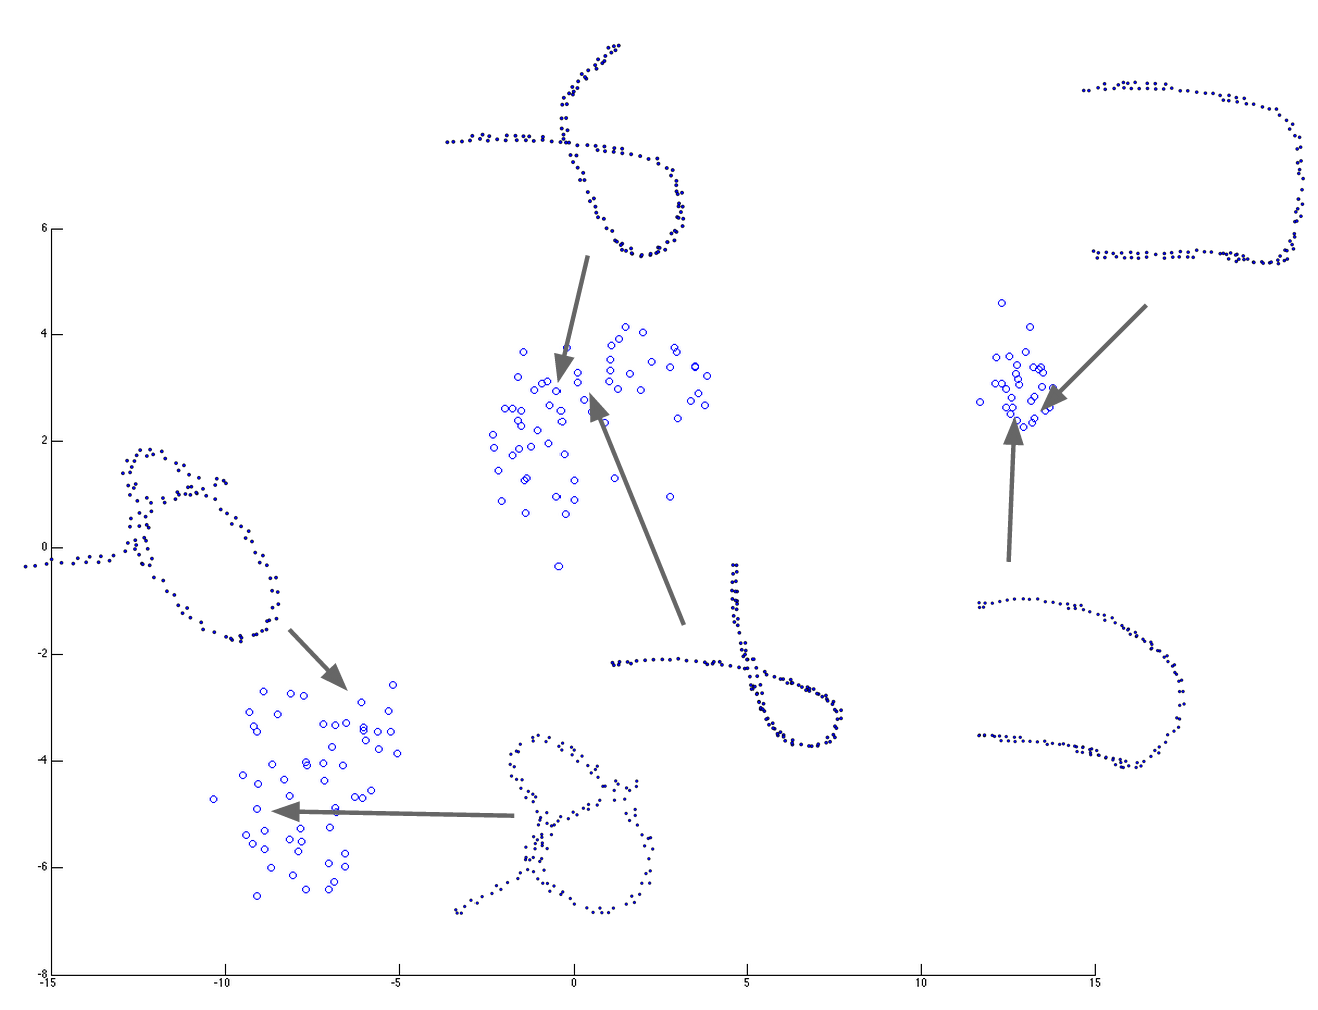
\includegraphics[width=0.5\textwidth]{tsne_clusters}
\caption{Two-dimensional t-SNE of rope configurations.}
\label{fig:tsne_clusters}
\end{figure}

In addition to directly solving for a scene registration and feasible trajectory, optimizing to perform trajectory transfer also yields useful information, which can be utilized to further improve the robustness of manipulation tasks. In particular, we can make use of the TPS registration error, which appears as a term in our optimization objective, as a tool to organize demonstrations into logical clusters.

The registration error provides a distance metric with which we can evaluate the similarity of scene configurations. This means that by using any kernel such as a Gaussian RBF, we can run a kernelized $k$-means clustering algorithm~\cite{Dhillon2004} to separate the start configurations of demonstrations into distinct clusters. Thus, in our current optimization framework, we need only set a few additional parameters (the number of clusters and the parameters of the kernel function) to derive structure from known scene configurations and demonstrations. In effect, we are grouping specific scene configurations into $k$ well-known, commonly encountered abstract states, and the provided demonstrations then constitute transitions between these states.

For a knot-tying scenario, in which a robot attempts to autonomously tie a knot, visualizing these clusters using a low-dimensional embedding such as t-SNE~\cite{tSNE2008} demonstrates that the registration error as a similarity metric is able to effectively separate the scene configurations into three clusters, as shown in Figure~\ref{fig:tsne_clusters}. Additionally, examining the rope configurations present within each cluster indicates that each cluster represents a distinct step along this particular rope-tying method.

These clusters also provide us an effective means of quantifying how effectively we can proceed from a given state. For a new scene configuration, we can find its $k$ nearest neighbors out of the provided demonstration start configurations. We then create a histogram of the clusters of these $k$ demonstrations, and take the maximum count as a score. We call this score the \emph{consensus score} and use it as a measure of how likely we are to succeed from a given scene configuration. Intuitively, a higher consensus score is better because it is easier to generalize to scene configurations that lie in the interior of clusters. For configurations that satisfy this property, there exist many demonstrations that operate on similar configurations, which indicates that this configuration is not extraordinary or unexpected and provides many valid demonstrations to choose from. On the other hand, points that are far away from these clusters are troublesome, since none of the existing demonstrations operate on similar configurations.

Applying this is simple, then. To evaluate a possible demonstration, we apply the demonstration to the current scene in simulation, then examine the resulting state. If this state has a high consensus score, then it is a well-understood state, and this demonstration is a viable execution candidate; otherwise, if the state has a low consensus score, then it is likely to lead to an unrecoverable configuration, and should be avoided. We found that in very challenging settings, where the rope configuration differs greatly from those of the demonstrations, implementing this simple method improved the success rate by as much as 20%.

%If we allow ourselves to assume domain-specific knowledge, we can leverage this clustering to steer ourselves towards rope configurations that are well covered by demonstrations. In particular, if we have access to a rudimentary simulation of the test environment, then we can perform lookahead to avoid states that are poorly understood. Given a set of demonstrations to generalize, we can compute nearest-neighbors using registration cost as a similarity measure. If a state's highest ranked nearest neighbors all belong to the same cluster, we say there is a high consensus score for that state. If the consensus score is below some threshold, we can simulate candidates and take the demonstration which, after simulation, has the highest consensus score. In applying this heuristic, we bias our search to stay on the interior of our learned clusters. In practice, we found that there were many scenarios where this heuristic was able to avoid dead ends that blocked nearest-neighbor. Figure~\ref{fig:lookahead_results} illustrates one such scenario. Note that simply using minimum or mean registration cost as a search heuristic will likely lead to failure: there are many cases where executing the best demonstration (the demonstration that leads to tying a knot in the fewest steps) yields a higher registration cost than an alternative. 

\begin{figure}
\centering
\begin{subfigure}[b]{.24\textwidth}
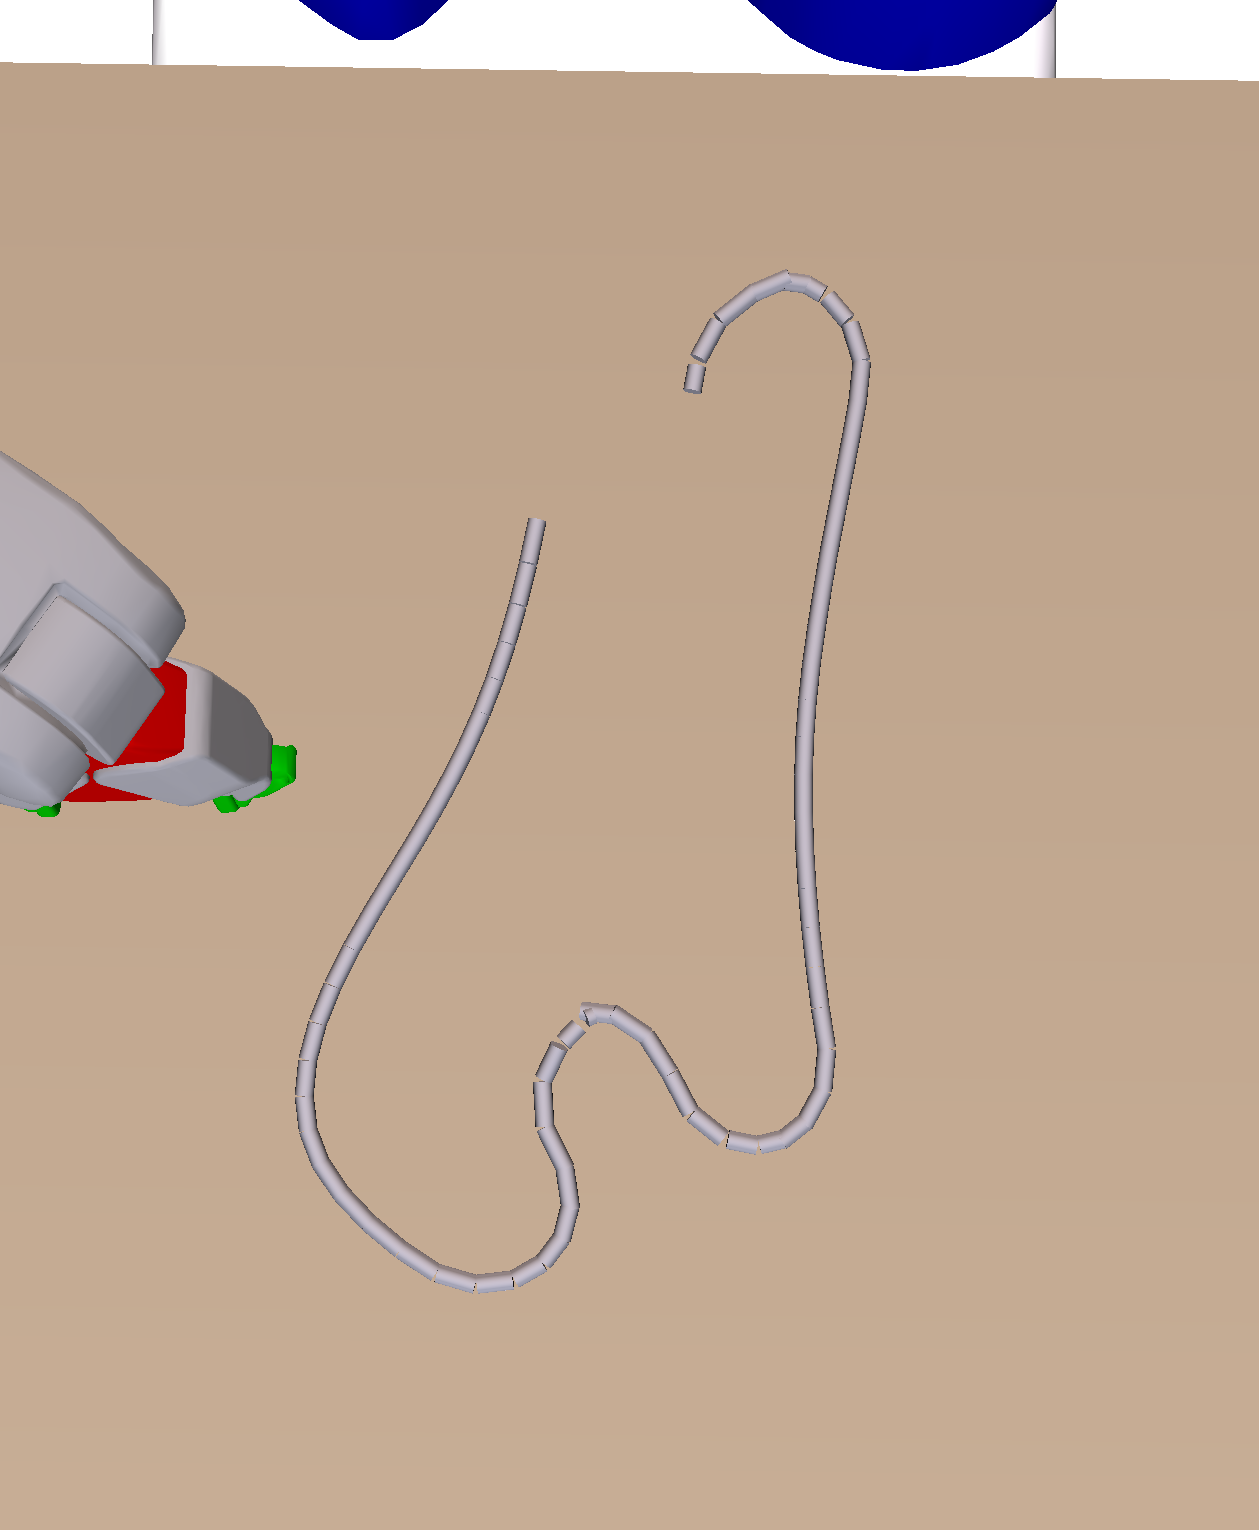
\includegraphics[width=\textwidth]{no_lookahead_fail_start.png}
\caption{}
\end{subfigure}
\begin{subfigure}[b]{.24\textwidth}
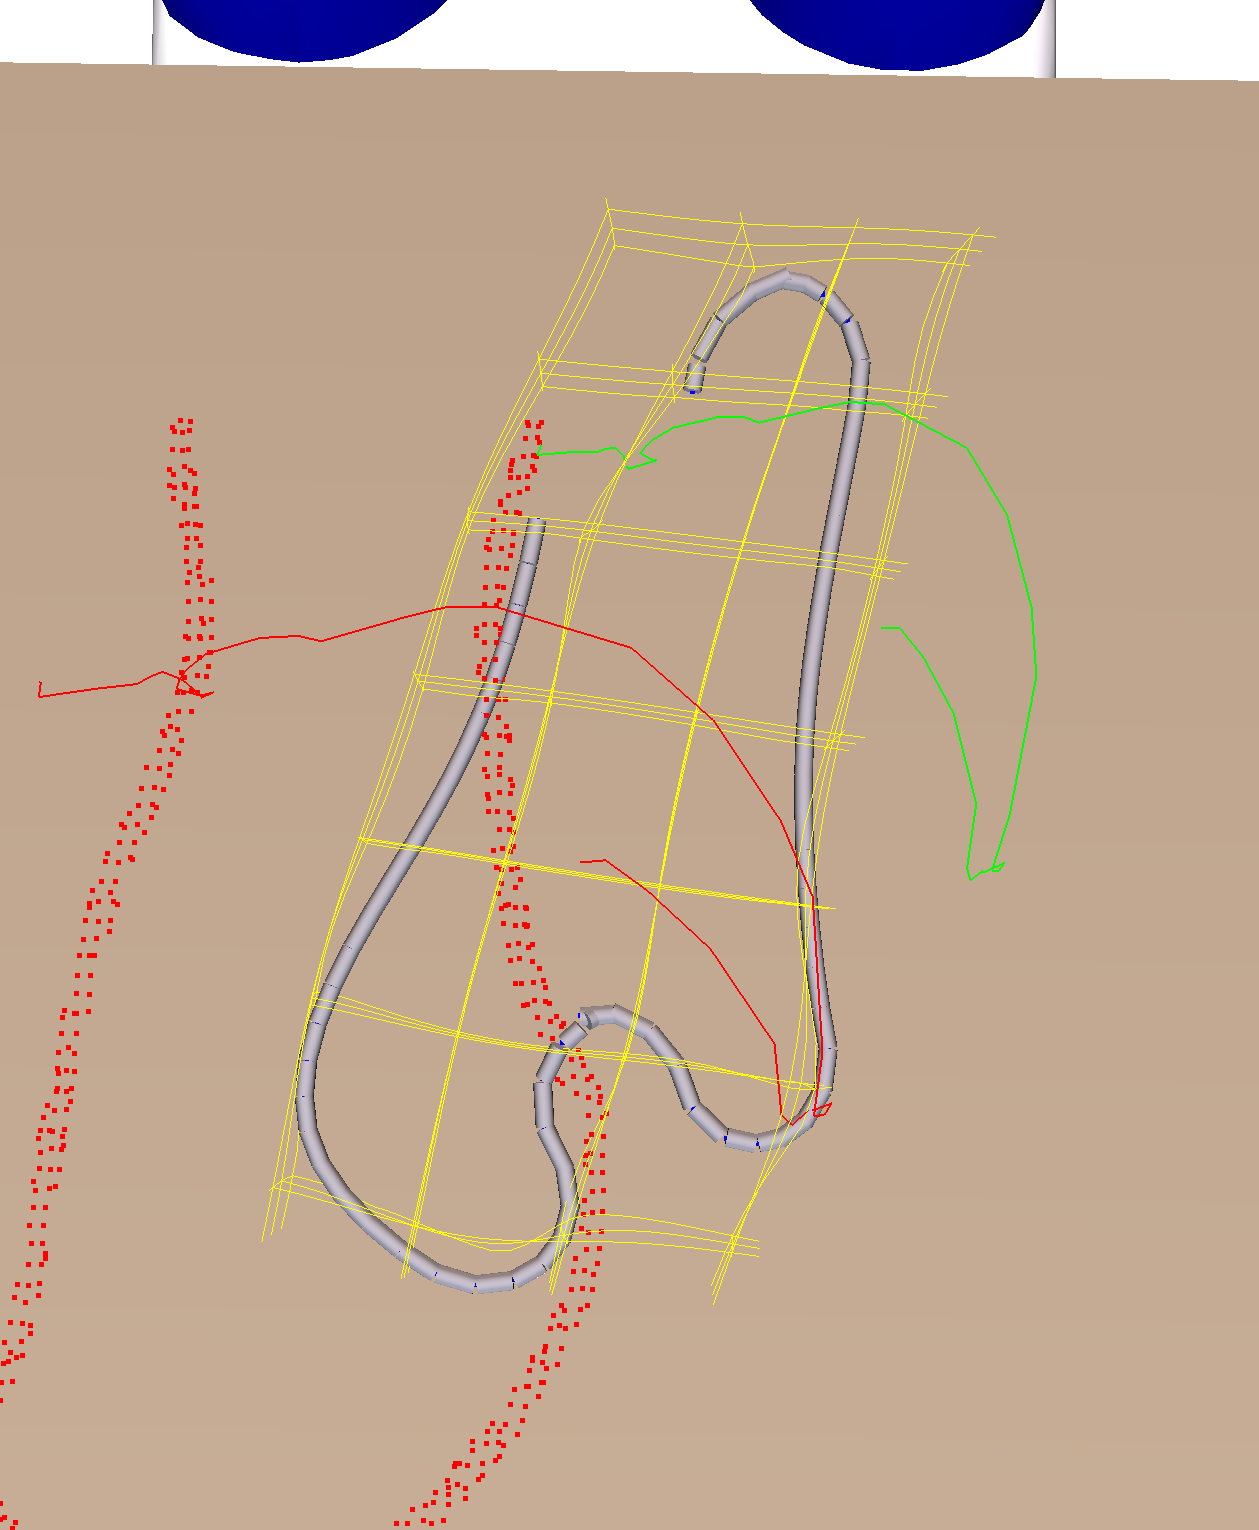
\includegraphics[width=\textwidth]{sim_res1.png}
\caption{}
\end{subfigure}
\begin{subfigure}[b]{.24\textwidth}
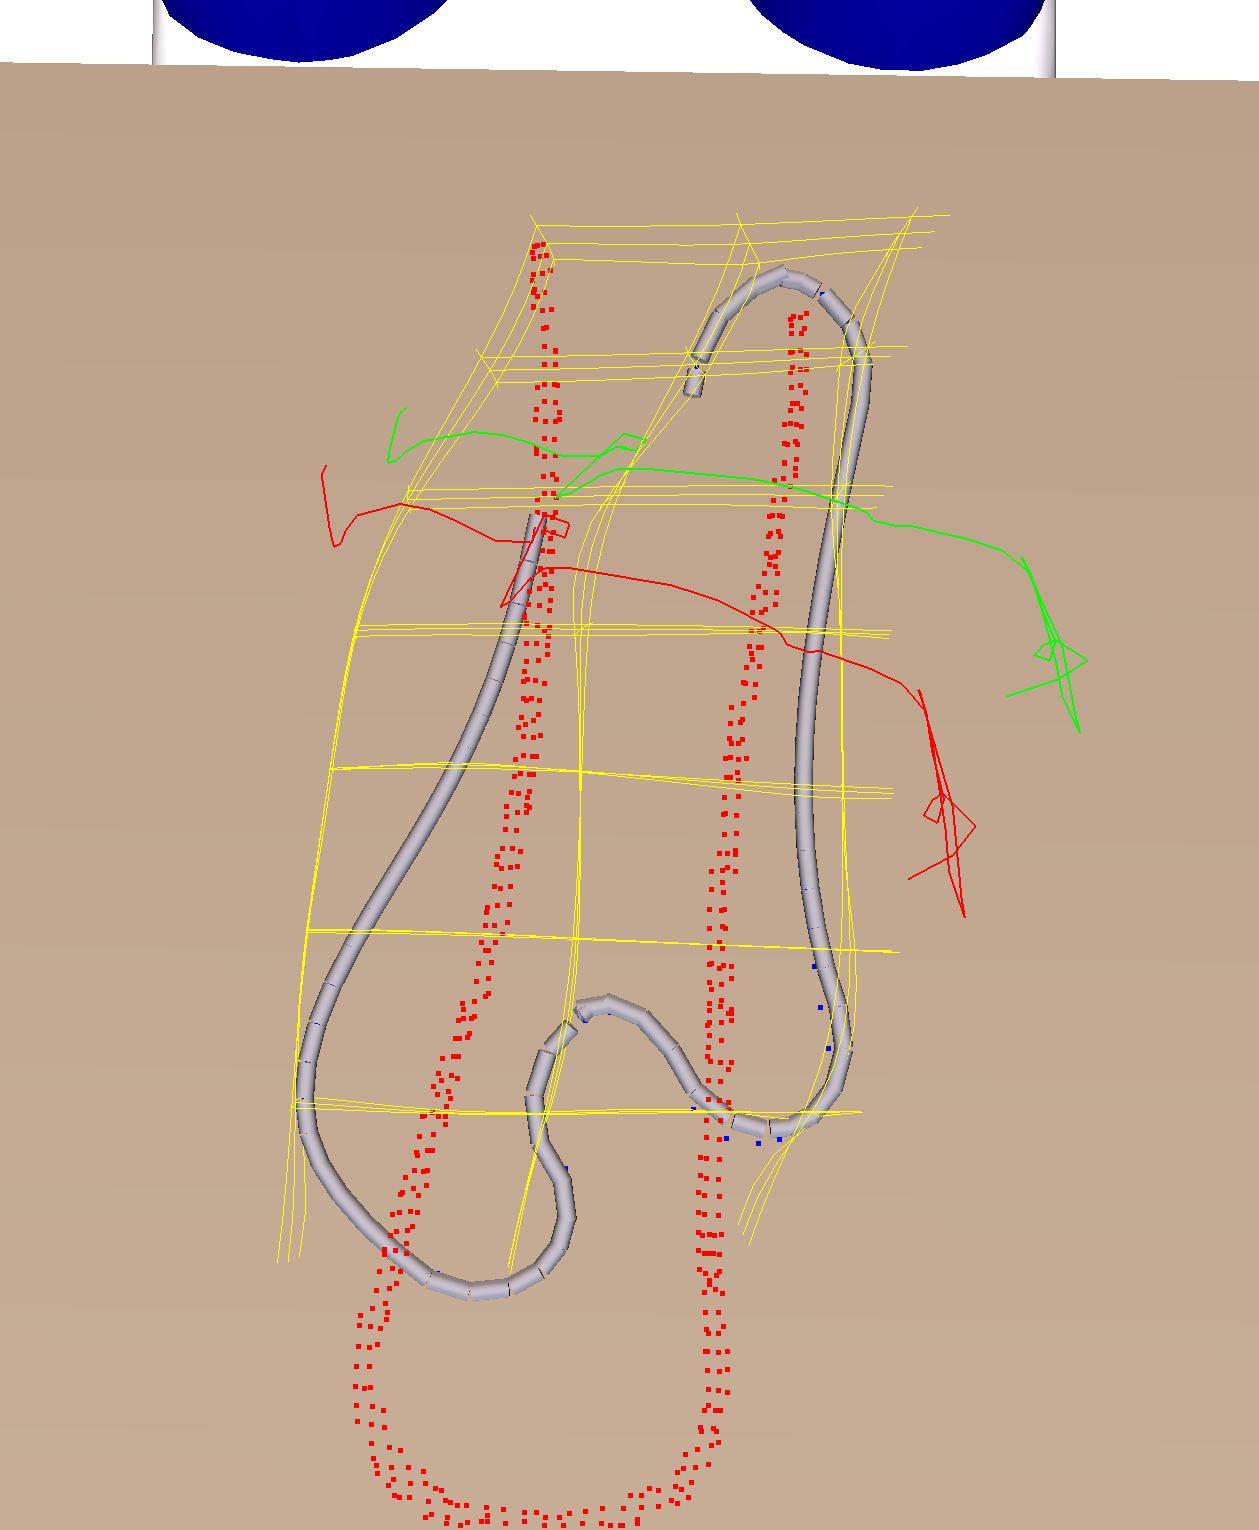
\includegraphics[width=\textwidth]{sim_res2.png}
\caption{}
\end{subfigure}
\begin{subfigure}[b]{.24\textwidth}
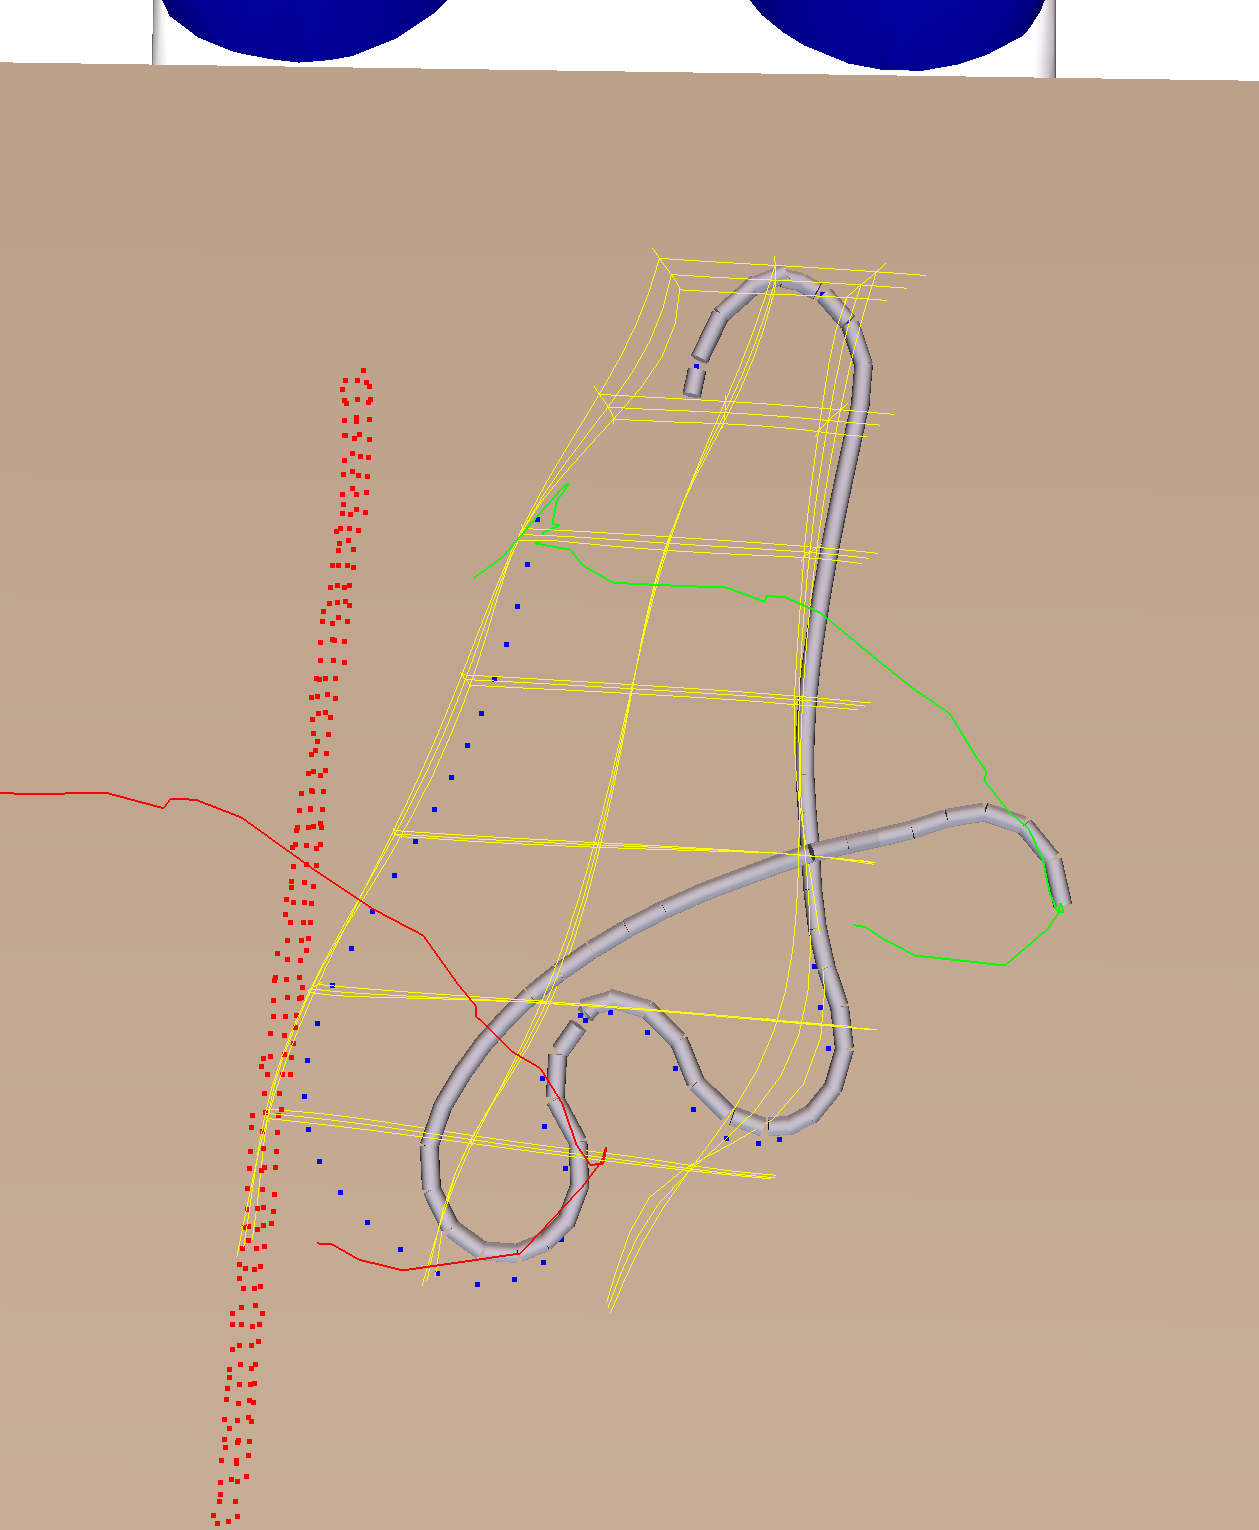
\includegraphics[width=\textwidth]{sim_res3.png}
\caption{}
\end{subfigure}\\
\caption{(a): Initial state for a simulation run where lookahead succeeds, but nearest-neighbor does not. (b)-(c): States that result from simulating the two best nearest neighbors according to registration cost. The green path illustrates the path the gripper took. It misses the rope entirely, so the next state is the same as the initial state. (d): Simulation result from using the 3rd best demonstration according to registration cost. This demonstration is the one chosen by our heuristic and results in a successful knot-tie.}
\label{fig:lookahead_results}
\end{figure}

\section{Limitations and Future Work}

We are currently implementing our unified objective for simulations of three-dimensional tasks, in particular rope-tying and suturing. Our hope is that this will either provide convincing evidence that the unified formulation produces and selects better trajectories, or it will provide new insight with which we can revise our approach. In addition, to formally incorporate normals into the optimization, we are implementing the previously-described reformulation of the TPS objective that incorporates first-order constraints~\cite{BooksteinGreen}.

We also plan to further investigate potential applications of the TPS registration error (from our unified optimization) to increasing the robustness of learning from demonstrations. For instance, we can use reinforcement learning or inverse reinforcement learning to learn a Q-function for each action, in which the space of actions is a discrete set with a one-to-one correspondence between actions and demonstrations. This would enable us to learn which demonstrations generalize well and discover, on a per demonstration basis, which rope states each demonstration is most applicable to.

%There is also an interesting avenue of research based on a more explicit modelling of the underlying MDP that our robot is acting in. In this setting, the state space is the set of paired configurations of the robot and rope. The space of actions is a discrete set, with one action corresponding to each demonstration. This formalism lets us apply techniques such as reinforcement learning or inverse reinforcement learning to learn a Q-function for each action. Such approaches would enable us to learn which demonstrations generalize well and discover, on a per demonstration basis, which rope states each demonstration is most applicable to.

%Estimating scene correspondences more accurately is also crucial for improving demonstration selection. Schulman et al. use the TPS-RPM approach to estimate correspondences between point clouds of the demonstration scene and the new scene. TPS-RPM only takes into account the positions of the points, and requires a one-to-one correspondence between the points in the two point clouds. However, there may be outliers, points in the demonstration scene that do not correspond to any in the new scene or vice versa. Using computer-vision based features, such as SIFT and shape contexts, has the potential to detect these outliers and improve estimation of point correspondences.

\section{Conclusion}

We have presented a unified optimization approach that improves the robustness of trajectory transfer by jointly optimizing for both a smooth warping function and a feasible trajectory. In addition, we explored incorporating surface normal correspondences to account for crucial scene geometry information that the existing state-of-the-art method ignores. We have provided examples which convincingly demonstrate that our proposed extensions improve robustness of the trajectory transfer method. Finally, we show that by clustering states based on registration error (a term in our objective function), we can avoid areas of the state space that are poorly explored, thus improving the robustness of learning from multiple demonstrations.

% We have presented several approaches for improving the transfer of trajectories to new scenarios when multiple demonstrations are available. We improve the robustness of trajectory transfer by jointly optimizing for both a smooth warping function and a feasible trajectory, as well as incorporating surface normal correspondences. Leveraging clustering allows us to use lookahead to predict how likely applying a certain transferred trajectory will result in success, which improves demonstration selection. Finally, we have provided examples which convincingly demonstrate that our proposed extensions improve robustness of the trajectory transfer method.

\bibliographystyle{unsrt}
\bibliography{references}

\end{document}

